% Template for Cogsci submission with R Markdown

% Stuff changed from original Markdown PLOS Template
\documentclass[10pt, letterpaper]{article}

\usepackage{cogsci}
\usepackage{pslatex}
\usepackage{float}
\usepackage{caption}

% amsmath package, useful for mathematical formulas
\usepackage{amsmath}

% amssymb package, useful for mathematical symbols
\usepackage{amssymb}

% hyperref package, useful for hyperlinks
\usepackage{hyperref}

% graphicx package, useful for including eps and pdf graphics
% include graphics with the command \includegraphics
\usepackage{graphicx}

% Sweave(-like)
\usepackage{fancyvrb}
\DefineVerbatimEnvironment{Sinput}{Verbatim}{fontshape=sl}
\DefineVerbatimEnvironment{Soutput}{Verbatim}{}
\DefineVerbatimEnvironment{Scode}{Verbatim}{fontshape=sl}
\newenvironment{Schunk}{}{}
\DefineVerbatimEnvironment{Code}{Verbatim}{}
\DefineVerbatimEnvironment{CodeInput}{Verbatim}{fontshape=sl}
\DefineVerbatimEnvironment{CodeOutput}{Verbatim}{}
\newenvironment{CodeChunk}{}{}

% cite package, to clean up citations in the main text. Do not remove.
\usepackage{apacite}

% KM added 1/4/18 to allow control of blind submission


\usepackage{color}

% Use doublespacing - comment out for single spacing
%\usepackage{setspace}
%\doublespacing


% % Text layout
% \topmargin 0.0cm
% \oddsidemargin 0.5cm
% \evensidemargin 0.5cm
% \textwidth 16cm
% \textheight 21cm

\title{Intuitive archeology: Reasoning about social transmission of artifacts'
designs}


\author{{\large \bf Ethan S. Hurwitz (ehurwitz@ucsd.edu)}, {\large \bf Timothy F. Brady (timbrady@ucsd.edu)}, \\ {\large \bf Adena Schachner (adschachner@ucsd.edu)} \\ University of California, San Diego, Department of Psychology \\ 9500 Gilman Drive M/C 0109, San Diego, CA 92093-0109 USA}

\begin{document}

\maketitle

\begin{abstract}
Include no author information in the initial submission, to facilitate
blind review. The abstract should be one paragraph, indented 1/8 inch on
both sides, in 9\textasciitilde{}point font with single spacing. The
heading `Abstract' should be 10\textasciitilde{}point, bold, centered,
with one line of space below it. This one-paragraph abstract section is
required only for standard six page proceedings papers. Following the
abstract should be a blank line, followed by the header `Keywords' and a
list of descriptive keywords separated by semicolons, all in
9\textasciitilde{}point font, as shown below.

\textbf{Keywords:}
social cognition; Bayesian inference; explanation; social transmission;
imitation; artifact; design
\end{abstract}

\section{General Formatting
Instructions}\label{general-formatting-instructions}

For general information about authoring in markdown, see
\textbf{\href{http://rmarkdown.rstudio.com/authoring_basics.html}{here}.}

The entire content of a paper (including figures, references, and
anything else) can be no longer than six pages in the
\textbf{initial submission}. In the \textbf{final submission}, the text
of the paper, including an author line, must fit on six pages. Up to one
additional page can be used for acknowledgements and references.

The text of the paper should be formatted in two columns with an overall
width of 7 inches (17.8 cm) and length of 9.25 inches (23.5 cm), with
0.25 inches between the columns. Leave two line spaces between the last
author listed and the text of the paper; the text of the paper (starting
with the abstract) should begin no less than 2.75 inches below the top
of the page. The left margin should be 0.75 inches and the top margin
should be 1 inch. \textbf{The right and bottom margins will depend on
whether you use U.S. letter or A4 paper, so you must be sure to
measure the width of the printed text.} Use 10\textasciitilde{}point
Times Roman with 12\textasciitilde{}point vertical spacing, unless
otherwise specified.

The title should be in 14\textasciitilde{}point bold font, centered. The
title should be formatted with initial caps (the first letter of content
words capitalized and the rest lower case). In the initial submission,
the phrase ``Anonymous CogSci submission'' should appear below the
title, centered, in 11\textasciitilde{}point bold font. In the final
submission, each author's name should appear on a separate line,
11\textasciitilde{}point bold, and centered, with the author's email
address in parentheses. Under each author's name list the author's
affiliation and postal address in ordinary 10\textasciitilde{}point
type.

Indent the first line of each paragraph by 1/8\textasciitilde{}inch
(except for the first paragraph of a new section). Do not add extra
vertical space between paragraphs.

\section{Method}\label{method}

\subsection{Design}\label{design}

Participants were shown tools that two target individuals designed and
were asked to judge whether or not one of those individuals copied the
other's tool. The participants were given the following scenario: Two
people at a time were given a puzzle box to solve. The puzzle box has a
button in it that plays music. The goal is to push the button, but
there's no way to reach it. The box is glued shut and doesn't open. The
only way in is through an opening at the top of the box. Each person was
asked to build a tool that could reach the button. The tools were built
by combining a handle piece with a rod piece. \(figure?\) Some people
had 10 different handles to choose from while others only had two.
Additionally, some people had 10 rods to choose from while others only
had 2. Further, some individuals were trying to solve a puzzle box with
a circular opening which all the rod pieces could fit through. Others
were trying to solve a puzzle box with a star-shaped opening which only
the star shaped rod could fit through. While designing the tools the
people were seated in the same room. While facing away from each other
they could easily turn around to see what the other person was making,
or complete the task without turning around and looking at the other
person's tool.

We parametrically manipulated: 1. the number of rod and handle options
available to the designers when constructing their tools (2 versus 10
options available for each). 2. The presence or absence of a functional
constraint, imposed by the structure of the puzzle they were trying to
solve (i.e.~whether they were trying to solve the circle box or star
box). 3. The extent of similarity of the two tools that were built
(perceptual similarity) - the two tools that are built are either
identical on both of the two parts (rod and handle are the same), on 1
part (rod or handle are the same), or on 0 parts (both rod and handle
are different). This resulted in 24 unique trials.

\subsection{Procedure}\label{procedure}

Individuals who opted to participate were presented a URL to link to the
experiment. Links were anonymized and collected no identifying
information (i.e., IP address). The experiment was hosted on Qualtrics
(www.Qualtrics.com), an online survey and experiment administration
website. Through it's security and privacy features, Qualtrics is a
suitable platform for anonymous data collection and storage. Each
participant completed a randomly presented subset of 4 unique trials out
of the 24 total. Within each trial was one randomly selected attention
check question out of 3 possibilities, assessing either what puzzle box
the people were trying to solve, how many rod options they had, or how
many handle options they had. After these 4 trials, there were 4 memory
check questions, assessing memory for the instructions regarding which
rod and handle options could be used to successfully solve each of the
two puzzle boxes. There were also two free response questions asking
participants to recall what they did throughout the experiment and what
they thought it was about. Finally, there were some questions assessing
demographics \(and English proficiency\).

\subsection{Participants}\label{participants}

The study was approved by the Institutional Review Board of the
University of California, San Diego. All participants gave their
informed consent before beginning study procedures. A pilot dataset with
a slightly different design (within-subject and a subset of the current
trials) was used to conduct a power analysis with the R ``pwr'' package
(Champely et al., 2018). A paired t-test power calculation was conducted
on participant-level BICs. Results revealed that with our current design
we would need 18 data points per trial to have .90 power at an error
probability of alpha = .05. With each participant completing 4 trials,
106 adults (56 male, 49 female, 1 other gender identity; mean age =
37.87, SD = 10.9, range = 20 - 72) were recruited through Amazon's
Mechanical Turk (MTurk). Previous work has shown that samples recruited
through MTurk are equally, if not more, representative of the general
population (Berinsky, Huber, \& Lenz, 2012). Participants were all from
the United States, had not previously completed this or any similar
experiments, and were paid \texttt{\$}1.10 for their time (mean
participation time = 8.31 minutes).

\subsubsection{Data exclusion}\label{data-exclusion}

Participants were excluded from analysis if any of the following
criterion were met: 1. If they were assessed to be a non-native English
speaker or appeared to be a bot/non-human \((n = 13)\). To make this
assessment, two native-English speakers coded participants' free
response answers to flag individuals suspected of being either a
non-native English speaker or a bot/non-human. Participants marked by
only one coder were subsequently discussed by both coders to reach an
agreement. These coders did not have access to participants' other data,
and thus were not able to exclude individuals providing data which was
counter-hypothesis. 2. Any of the four memory check questions were
answered incorrectly \((n = 49)\). 3. At least half of the within-trial
attention check questions were answered incorrectly \((n = 12)\). 4.
Having previously participated in the experiment \((n = 1)\). Additional
participants were recruited to replace those who were excluded to reach
our target of 106 participants.

\subsection{Data analysis}\label{data-analysis}

Four Bayesian models were compared to assess which best predicts
participants' responses: 1. A model which represents explanation-based
reasoning: here, both the number of available options and functional
constraint of the puzzle box type are considered and influence copy
assessments. 2. A model that does not take into consideration the
functional constraint of the box type (Ignore Star Constraint or ISC
model). 3. A model that does not take into consideration the number of
options to choose from (n Imagined Choices or nIC model). 4. A model
that does not take into consideration both the number of options to
choose from and the functional constraint of the box type (Ignore Star
Constraint n Imagined Choices or ICSnIC model). See the supplementary
materials for all model code.

For each model, the best fitting parameters and likelihood of our data
given those parameters were assessed via maximum likelihood estimation
(MLE). MLE searches a prespecified space of possible parameter values,
often all possible/likely values, to assess the likelihood of your data
given each value of each parameter being fit. It then returns the
specific parameter values which maximize this likelihood. Tables 1 and 2
respectively summarize the lower and upper bounds of our parameter
search space and the MLE-derived likelihood maximizing parameter values.

\begin{table}[H]
\centering
\begin{tabular}{rlrr}
  \hline
 & Parameter & Lower.Bounds & Upper.Bounds \\ 
  \hline
1 & Copying Prior & 0.00 & 1.00 \\ 
  2 & Copying Error Rate & 1.00 & Inf \\ 
  3 & Number of Choices & 0.00 & 0.10 \\ 
   \hline
\end{tabular}
\caption{Bounds of parameter value search space.} 
\end{table}

\begin{table}[H]
\centering
\begin{tabular}{rlrrr}
  \hline
 & Model & Best.Prior & Best.Error.Rate & Best.nChoice \\ 
  \hline
1 & Full & 0.09 & 0.10 &  \\ 
  2 & ISC & 0.06 & 0.10 &  \\ 
  3 & nIC & 0.09 & 0.10 & 5.23 \\ 
  4 & ISCnIC & 0.12 & 0.10 & 2.71 \\ 
   \hline
\end{tabular}
\caption{MLE-derived best fitting parameters.} 
\end{table}

Bayesian information criterion (BIC) will be used to assess model fit
and compare fit between competing models (Schwarz, 1978). BIC uses
deviance to assess model fit in a way similar to using sum of squares of
residuals in ordinary least squares. However, to compensate for
potential overfitting, BIC proportionally penalizes models for both the
number of parameters and data points fit. Thus, greater BICs correspond
to a worse fitting model. Guidelines provided by Kass and Raferty (1995)
were used in comparing model fit. In particular, BIC differences of
between \(2 - 6\) are taken as positive evidence of a better fit of the
model with the smaller BIC, between \(6 - 10\) taken as strong evidence,
and 10 or greater as decisive evidence. To estimate their accuracy, we
calculated standard errors (SEs) for each BIC. These SEs were derived
via bootstrapping. Specifically, we boostrapped many samples from our
data (sampling with replacement) and calculated a BIC for each
bootstrapped sample, generating a distribution of possible BICs. This
BIC distribution was used to find the SEs of our experimentally attained
BICs.

\section{Results}\label{results}

\section{Formalities, Footnotes, and
Floats}\label{formalities-footnotes-and-floats}

Use standard APA citation format. Citations within the text should
include the author's last name and year. If the authors' names are
included in the sentence, place only the year in parentheses, as in
(1972), but otherwise place the entire reference in parentheses with the
authors and year separated by a comma (Newell \& Simon, 1972). List
multiple references alphabetically and separate them by semicolons
(Chalnick \& Billman, 1988; Newell \& Simon, 1972). Use the et. al.
construction only after listing all the authors to a publication in an
earlier reference and for citations with four or more authors.

For more information on citations in RMarkdown, see
\textbf{\href{http://rmarkdown.rstudio.com/authoring_bibliographies_and_citations.html\#citations}{here}.}

\subsection{Footnotes}\label{footnotes}

Indicate footnotes with a number\footnote{Sample of the first
footnote.} in the text. Place the footnotes in 9 point type at the
bottom of the page on which they appear. Precede the footnote with a
horizontal rule.\footnote{Sample of the second footnote.} You can also
use markdown formatting to include footnotes using this
syntax.\footnote{Sample of a markdown footnote.}

\subsection{Figures}\label{figures}

All artwork must be very dark for purposes of reproduction and should
not be hand drawn. Number figures sequentially, placing the figure
number and caption, in 10 point, after the figure with one line space
above the caption and one line space below it. If necessary, leave extra
white space at the bottom of the page to avoid splitting the figure and
figure caption. You may float figures to the top or bottom of a column,
or set wide figures across both columns.

\subsection{Two-column images}\label{two-column-images}

You can read local images using png package for example and plot it like
a regular plot using grid.raster from the grid package. With this method
you have full control of the size of your image. \textbf{Note: Image
must be in .png file format for the readPNG function to work.}

You might want to display a wide figure across both columns. To do this,
you change the \texttt{fig.env} chunk option to \texttt{figure*}. To
align the image in the center of the page, set \texttt{fig.align} option
to \texttt{center}. To format the width of your caption text, you set
the \texttt{num.cols.cap} option to \texttt{2}.

\begin{CodeChunk}
\begin{figure*}[h]

{\centering 
\includegraphics{figs/2-col-image-1} 

}

\caption[This image spans both columns]{This image spans both columns. And the caption text is limited to 0.8 of the width of the document.}\label{fig:2-col-image}
\end{figure*}
\end{CodeChunk}

\subsection{One-column images}\label{one-column-images}

Single column is the default option, but if you want set it explicitly,
set \texttt{fig.env} to \texttt{figure}. Notice that the
\texttt{num.cols} option for the caption width is set to \texttt{1}.

\begin{CodeChunk}
\begin{figure}[H]

{\centering 
\includegraphics{figs/image-1} 

}

\caption[One column image]{One column image.}\label{fig:image}
\end{figure}
\end{CodeChunk}

\subsection{R Plots}\label{r-plots}

You can use R chunks directly to plot graphs. And you can use latex
floats in the fig.pos chunk option to have more control over the
location of your plot on the page. For more information on latex
placement specifiers see
\textbf{\href{https://en.wikibooks.org/wiki/LaTeX/Floats,_Figures_and_Captions}{here}}

\begin{CodeChunk}
\begin{figure}[H]

{\centering 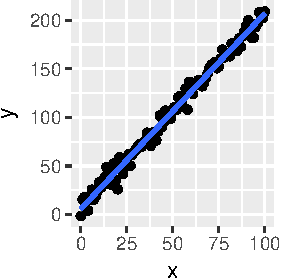
\includegraphics{figs/plot-1} 

}

\caption[R plot]{R plot}\label{fig:plot}
\end{figure}
\end{CodeChunk}

\subsection{Tables}\label{tables}

Number tables consecutively; place the table number and title (in 10
point) above the table with one line space above the caption and one
line space below it, as in Table 1. You may float tables to the top or
bottom of a column, set wide tables across both columns.

You can use the xtable function in the xtable package.

\begin{table}[H]
\centering
\begin{tabular}{rrrrr}
  \hline
 & Estimate & Std. Error & t value & Pr($>$$|$t$|$) \\ 
  \hline
(Intercept) & -0.10 & 0.10 & -1.0 & 0.33 \\ 
  x & 2.05 & 0.10 & 21.6 & 0.00 \\ 
   \hline
\end{tabular}
\caption{This table prints across one column.} 
\end{table}

\section{Acknowledgements}\label{acknowledgements}

Place acknowledgments (including funding information) in a section at
the end of the paper.

\section{References}\label{references}

\setlength{\parindent}{-0.1in} \setlength{\leftskip}{0.125in} \noindent

\hypertarget{refs}{}
\hypertarget{ref-berinskyEvaluatingOnlineLabor2012}{}
Berinsky, A. J., Huber, G. A., \& Lenz, G. S. (2012). Evaluating online
labor markets for experimental research: Amazon. com's Mechanical Turk.
\emph{Political Analysis}, \emph{20}(3), 351--368.

\hypertarget{ref-ChalnickBillman1988a}{}
Chalnick, A., \& Billman, D. (1988). Unsupervised learning of
correlational structure. In \emph{Proceedings of the tenth annual
conference of the cognitive science society} (pp. 510--516). Hillsdale,
NJ: Lawrence Erlbaum Associates.

\hypertarget{ref-champelyPwrBasicFunctions2018}{}
Champely, S., Ekstrom, C., Dalgaard, P., Gill, J., Weibelzahl, S.,
Anandkumar, A., \ldots{} Rosario, H. D. (2018). Pwr: Basic Functions for
Power Analysis (Version 1.2-2). Retrieved from
\url{https://CRAN.R-project.org/package=pwr}

\hypertarget{ref-kassBayesFactors1995a}{}
Kass, R. E., \& Raftery, A. E. (1995). Bayes factors. \emph{Journal of
the American Statistical Association}, \emph{90}(430), 773--795.

\hypertarget{ref-NewellSimon1972a}{}
Newell, A., \& Simon, H. A. (1972). \emph{Human problem solving}.
Englewood Cliffs, NJ: Prentice-Hall.

\hypertarget{ref-schwarzEstimatingDimensionModel1978a}{}
Schwarz, G. (1978). Estimating the Dimension of a Model. \emph{The
Annals of Statistics}, \emph{6}(2), 461--464.
\url{http://doi.org/10.1214/aos/1176344136}

\bibliographystyle{apacite}


\end{document}
